%% ----------------------------------------------------------------
%% VideogularQuestions.tex
%% ----------------------------------------------------------------

\chapter{Videogular Questions} \label{Chapter:VideogularQuestions}

\begin{preamble}
	A \gls{Videogular} plugin was written to provide the core functionality of the project. It allows for questions to be overlaid on top of the video and handles user interaction. This plugin is called \gls{vgQuestions}. It also provides utility functions for the \gls{DF} messaging passing interface, making it easy to create content.
\end{preamble}

\section{Introduction}

This plugin was one of the primary focuses of the project, and is an accessible system presenting the user with questions overlaid on a video. A number of features were explicitly requested by the client, such as question types (\cref{Req:Question types}) and the ability to let users re-watch content easily if questions were answered incorrectly (\cref{Req:Jumping to content}).

\section{Design}

\begin{figure}[h]
	\makebox[\textwidth][c]{
		\begin{tikzpicture}[
			font=\sffamily,
			every matrix/.style={ampersand replacement=\&,column sep=1.6cm,row sep=1.6cm},
			source/.style={draw,thick,rounded corners,fill=yellow!20,inner sep=.3cm},
			vg-plugin/.style={draw,thick,rounded corners,fill=yellow!20,inner sep=.3cm},
			analytics-frontend/.style={draw,thick,rounded corners,fill=red!20,inner sep=.3cm},
			videogular/.style={draw,thick,circle,fill=blue!20},
			process/.style={draw,thick,circle,fill=blue!20},
			sink/.style={source,fill=green!20},
			datastore/.style={draw,very thick,shape=datastore,inner sep=.3cm},
			server/.style={source,fill=green!20},
			dots/.style={gray,scale=2},
			to/.style={->,>=stealth',shorten >=1pt,shorten <=1pt, semithick,font=\sffamily\footnotesize},
			between/.style={<->,>=stealth',shorten >=1pt,shorten <=1pt,semithick,font=\sffamily\footnotesize},
			every node/.style={align=center}]

			\matrix{
				\node[videogular] (videogular) {videogular}; \&
				\node[vg-plugin] (vg-questions) {vgQuestions}; \&
				\node[vg-plugin] (questions-worker) {questions-worker.js}; \&
				\node[server] (quiz) {quiz.js}; \\
			};

			\draw[to] (videogular.-20) --
				node[midway,below] {video states} (vg-questions.195);
			\draw[to] (vg-questions.-195) --
				node[midway,above] {command} (videogular.20);

			\draw[to] (vg-questions.-14) --
				node[midway,below] {user interactions} (questions-worker.190);
			\draw[to] (questions-worker.-190) --
				node[midway,above] {commands} (vg-questions.14);

			\draw[to] (questions-worker.-10) --
				node[midway,below] {utility function} (quiz.201); 
			\draw[to] (quiz.-201) --
				node[midway,above] {quiz description} (questions-worker.10);
		\end{tikzpicture}
	}
	\caption{The architecture of \gls{vgQuestions}}
	\label{Figure:vgquestions-architecture}
\end{figure}

The core of \gls{vgQuestions} is a \gls{DF} which defines the question sets. The \gls{DF} is loaded in a \gls{webworker} that will interact with \gls{vgQuestions} as shown in \autoref{Figure:vgquestions-architecture}. This uses a well-defined message passing interface to allow easy communication. Most users will not use the message passing interface and will instead use the authoring tool (see \autoref{Chapter:Authoring Tool}) to create a \gls{DF} that is run by the \gls{webworker}. This makes the plugin exceptionally flexible.

One of the issues discussed for this section was accessibility. It was decided that \gls{CSS} should be used for the styling to allow users to alter the styling to suit their needs. Keyboard accessibility would be an additional focus.

\section{Implementation}
The implementation of the questions overlay was split into three sections: first, representing the question sets internally; next, displaying the questions within the user interface; and finally, implementing the back-end communication between the question representations and the video.

\subsection{Annotations}
\label{Section:Annotations}

One of the main issues to address early on was how to represent the questions. The \gls{QTI} specification was investigated, but was found to be complicated and made implementing accessibility features difficult (see \autoref{Section:Reviewing Previous Work}). It was decided to design a new format for representing the data and logic that is used for a particular application of \gls{vgQuestions}.

This new format separates the front end of the library (responsible for interacting with the \gls{DOM}) from the data and logic describing the questions, by means of a message passing interface. This is achieved in a rigorous way in the browser by using a \gls{webworker}, a sandboxed thread that runs independently of other scripts, and without access to the \gls{DOM} or JavaScript functions which could compromise security. More information about their use within this project can be found in \autoref{Subsection:WebWorkers}.

Using JavaScript rather than a pure data representation (e.g. JSON or XML) allows the inclusion of logic to decide on an action to take (e.g. a question to display, or video location to skip to). This makes it extremely flexible and concise, and the isolation provided by the \gls{webworker} mitigates many security concerns with having an application that executes data given as input as code.

Every item in an \gls{annotation} can have an action and condition function. The action function is called when a item finishes, and is aware of the state of the \glspl{annotation}, allowing it to make decisions and affect the state of the video accordingly. For example, in \autoref{code:questionworker} this is used to show the ``skip back'' question only if the previous question is answered incorrectly.

The condition function is called to determine if the respective item will show. By default, when an \gls{annotation} is shown, each item is shown in sequence. However, if an item has a condition function the item only shown if the condition function returns \lstinline|true|. If the condition function returns \lstinline|false|, the item is skipped. This functionality is used in \autoref{code:questionworker} to have the video skip back on the request of the user.

An early decision was to define the difference between a poll and a quiz question. The decision made was that a poll is a type of quiz question that does not have a correct answer.

In the code this is captured in the \lstinline|record_response| attribute. If the \lstinline|record_response| attribute is set to \lstinline|true|, the question becomes a poll and sends the results to a server. If the \lstinline|correct_answer| attribute is set then the question has a correct answer which will be shown to the user, if requested. This allows a user to possible have a poll type question that stores the data collected and also has a right answer. This provides maximum flexibility, and the underlying code doesn't distinguish between a quiz or a poll.

Basic question types (single choice, multiple choice and scale questions) were implemented first. A variety of visualisations were implemented including check boxes, radio buttons and sliding scales. Validation was needed to ensure that the specified minimum and maximum limits were followed.

In reviewing the types of questions to support a class diagram was produced (\autoref{Figure:questions_class_diagram}) to describe the type of data that the questions would have. Once the additional question types of textual and range were implemented \cref{Req:Question types} was satisfied.

\begin{figure}
	\centering
	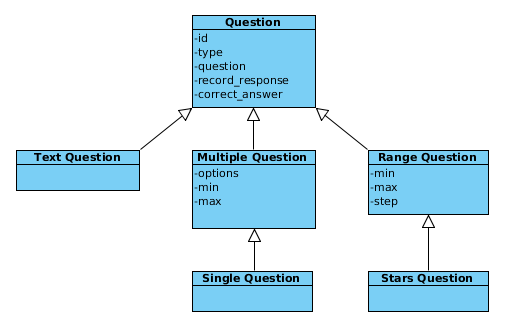
\includegraphics[width=12cm]{../figures/questions_class_diagram.png}
	\caption{A class diagram representing what attributes each question type needs}
	\label{Figure:questions_class_diagram}
\end{figure}

As seen in \autoref{Figure:questions_class_diagram} Single Question is a sub type of Multiple Question where min and max (the minimum and maximum selected number of answers) is 1. Similarly, the stars question is similar to the range question where the \lstinline|step value| is 1. These decisions were made to simplify the code to make a consistent interface easier to produce.

By having a standardised \gls{DF} that uses JavaScript functions, it was possible to write template functions that could be used by the authoring tool.

\subsection{Front-End and User Interface}

The appearance of the overlay depends on the question type to be shown. The layout of these different types was carefully considered for accessibility and ease of use. Mockups were made (see \cref{App:Question Mockups}) and user studies were done in collaboration with a third year project student (see \cref{App:User Study Results}).

A set of example \gls{CSS} files are supplied with the project that layout the questions according to the feedback received. Developers using any part of the project can use these styles as is, or modify/develop their own. The styles provided had a high contrast to meet the \gls{WCAG} 2.0 colour contrast standards. Keyboard accessibility was ensured throughout.

The final user interface produced can be viewed in \autoref{Figure:Screenshots/example poll}, \autoref{Figure:Screenshots/single question}, \autoref{Figure:Screenshots/multiple question}, \autoref{Figure:Screenshots/stars question}, \autoref{Figure:Screenshots/text question} and \autoref{Figure:Screenshots/range question}.

\subsection{Back-End - WebWorkers}
\label{Subsection:WebWorkers}

\Glspl{webworker} give a good way of running (sandboxed) background scripts that are computationally intensive. They are a way of multithreading - allowing multiple scripts to run simultaneously, avoiding the problem of unresponsive pages due to long running scripts. This is done by using message passing.

For example, when an answer is submitted by the user this would sent a message to the \gls{webworker} containing the answer. The \gls{webworker} can then process this information without affecting the responsiveness of the page. Once the processing is complete the \gls{webworker} can send a message back to the page to tell it what to do next.

\begin{figure}

\centering

\begin{sequencediagram}
	\newthread[white]{c}{Front End}
	\newinst[4]{s}{WebWorker}

	\mess{s}{annotations}{c}

	\stepcounter{seqlevel}
	\begin{call}
		{c}{annotationStart}
		{s}{showQuestion}
	\end{call}

	\stepcounter{seqlevel}
	\begin{call}
		{c}{questionResult}
		{s}{showQuestion}
	\end{call}

	\stepcounter{seqlevel}
	\begin{call}
		{c}{questionResult}
		{s}{endAnnotation}
	\end{call}
\end{sequencediagram}
\caption{Sequence diagram showing interactions between the front end and WebWorker}
\label{Figure:sequence_diagram_frontend_webworker}

\end{figure}

\autoref{Figure:sequence_diagram_frontend_webworker} illustrates messages that could pass between the \gls{webworker}, and the front end when the \autoref{code:questionworker} is used. Initially, the worker sends an \lstinline|annotationStart| message which contains the times which \glspl{annotation} will occur.

When the first time point is reached, the front end sends a \lstinline|annotationStart| message to the \gls{webworker} containing the \lstinline|id| of that \gls{annotation}. The worker then replies with a \lstinline|showQuestion| message containing the contents of the first question. Note that here the functions are not sent to the front end and it is just the JSON representation of the question is sent.

When the user responds to the question, that response is sent to the \gls{webworker} in a \lstinline|questionResult| message. In this case the user responded incorrectly, therefore when the \gls{webworker} evaluated the condition on the second question it evaluated to \lstinline|false|. This meant that the \gls{webworker} replied with another \lstinline|showQuestion| message.

Once the user responds to the second question, the response is again sent to the \gls{webworker}. In this case, this was the final question in the \gls{annotation}, so the \gls{webworker} responds with an \lstinline|endAnnotation| message.

\section{Summary}

An internal representation of the questions is given by the \gls{DF} that is used to display the questions to the user in the overlays. This allows all aspects of the questions presented to the user to be customised. This \gls{DF} can be manually written or it can be created by an authoring tool (\autoref{Chapter:Authoring Tool}).

\gls{CSS} was used to keep the appearance of the questions consistent and accessible but this also allows a developer to quickly change how the questions are shown with little technical knowledge of the system helping to fulfil \cref{Req:Use of colour}.

\Glspl{webworker} are used to communicate with the front end to provide the necessary messages for the expected actions to occur. By abstracting this to another thread utilisation of additional processing has been enabled and it is possible to ensure that the user has a better experience since the page is not as likely to freeze due to the additional thread sharing some of the processing. In addition, separating the front-end and back-end and only communicating via a message passing system provides low coupling which will allows customising one without affecting the other.
